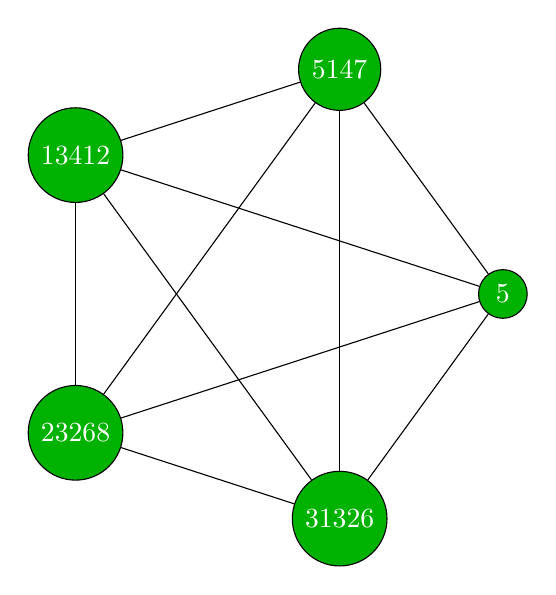
\begin{tikzpicture}
  \draw
    (0.000:3.000) node[fill=green!70!black, minimum size=4mm, circle, draw, text=white] (5){5}
    (72.000:3.000) node[fill=green!70!black, minimum size=2mm, circle, draw, text=white] (5147){5147}
    (144.000:3.000) node[fill=green!70!black, minimum size=2mm, circle, draw, text=white] (13412){13412}
    (216.000:3.000) node[fill=green!70!black, minimum size=2mm, circle, draw, text=white] (23268){23268}
    (288.000:3.000) node[fill=green!70!black, minimum size=2mm, circle, draw, text=white] (31326){31326};
  \begin{scope}[-]
    \draw (5) to (5147);
    \draw (5) to (13412);
    \draw (5) to (23268);
    \draw (5) to (31326);
    \draw (5147) to (13412);
    \draw (5147) to (23268);
    \draw (5147) to (31326);
    \draw (13412) to (23268);
    \draw (13412) to (31326);
    \draw (23268) to (31326);
  \end{scope}
\end{tikzpicture}
